\documentclass{cshwk}

\title{Wireshark Lab \#1, Intro}

\begin{document}

\maketitle

\section{Preperation}

Following the instructions, we used \texttt{wget} to retrieve an ASCII copy of *Alice in Wonderland* and stored it in \texttt{\~/Documents/alice.txt}.
\begin{verbatim}
    wget -O ~/Documents/alice.txt http://gaia.cs.umass.edu/wireshark-
    labs/alice.txt
\end{verbatim}
Next, we prevented the Large Send Offload (LSO) feature from interfering with the lab by running the following command:
\begin{verbatim}
    sudo ethtool -K wlp0s20f3 tso off gso off lro off
\end{verbatim}
To check the status of the LSO feature, we used the following command:
\begin{verbatim}
    sudo ethtool -k wlp0s20f3
\end{verbatim}

At last, we uploaded the file to the server as per the instructions, and the result is shown in Fig.~\ref{fig:Uploading}.


\begin{figure}[htbp]
    \centering
    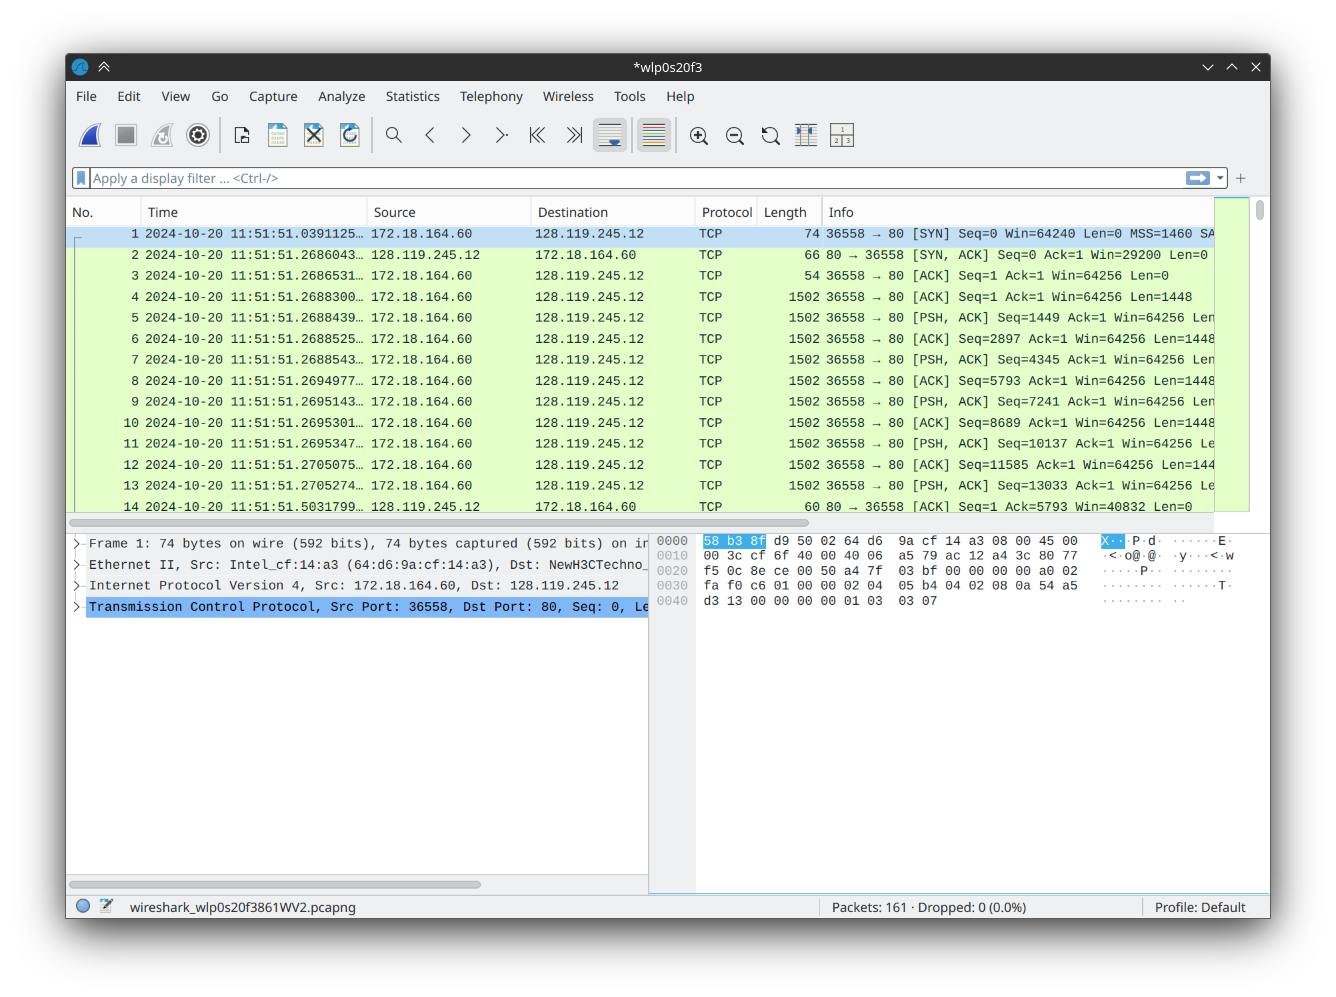
\includegraphics[width=0.6\textwidth]{./lab3-1.png}
    \caption{Uploading to the server}
    \label{fig:Uploading}
\end{figure}

\section{A first look at the captured trace}

\subsection*{Question 1.}
\begin{quote}
    What is the IP address and TCP port number used by the client computer (source) that is transferring the file to \href{http://giai.cs.umass.edu}{gaia.cs.umass.edu}?
\end{quote}

Inspecting the first three packets, we can observe the handshake process. By examining the \texttt{SYN} packet from the client, we can see that \textbf{the source IP address is \texttt{172.18.164.60} and the source port number is \texttt{36558}}. The details are shown in Fig.~\ref{fig:SYN}.


\begin{figure}[htbp]
    \centering
    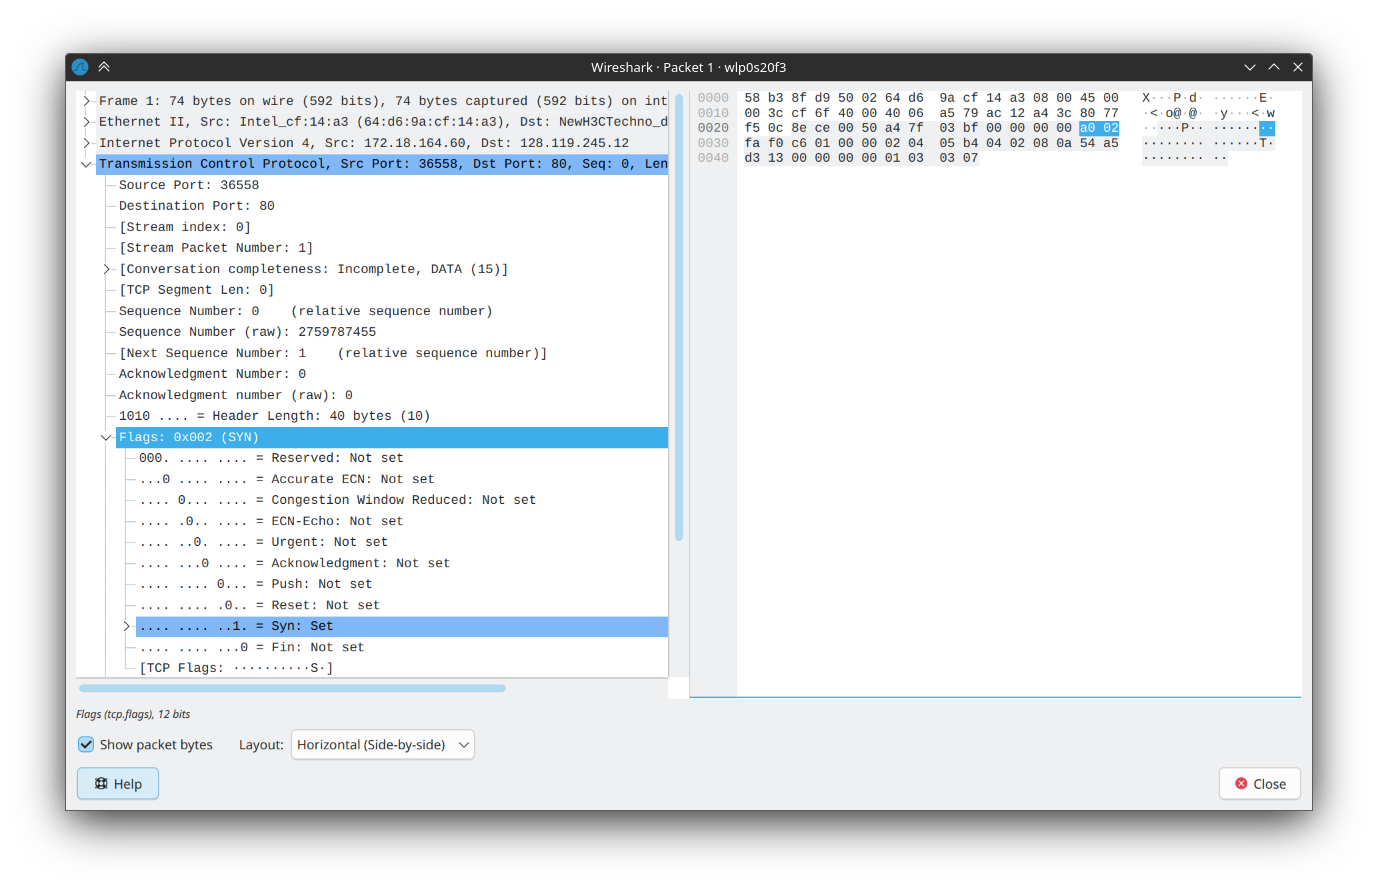
\includegraphics[width=0.8\textwidth]{./lab3-2.png}
    \caption{SYN packet}
    \label{fig:SYN}
\end{figure}

\subsection*{Question 2.}
\begin{quote}
    What is the IP address of \href{http://gaia.cs.umass.edu}{gaia.cs.umass.edu}? On what port number is it sending and receiving TCP segments for this connection?
\end{quote}

Also from Fig.~\ref{fig:SYN}, we can see the \textbf{destination IP address is \texttt{128.119.245.12} and the destination port number is \texttt{80}.}

\subsection*{Question 3.}
\begin{quote}
    What is the IP address and TCP port number used by your client computer (source) to transfer the file to gaia.cs.umass.edu?
\end{quote}

Question 3 is similar to Question 1. Inspect the \texttt{SYN} packet from the client, we can see \textbf{the source IP address is \texttt{172.18.164.60} and the source port number is \texttt{36558}}.

\section{TCP Basics}

\subsection*{Question 4.}
\begin{quote}
    What is the sequence number of the TCP SYN segment that is used to initiate the TCP connection between the client computer and gaia.cs.umass.edu? What is it in the segment that identifies the segment as a SYN segment?
\end{quote}

Also from Fig.~\ref{fig:SYN}, we can see the \textbf{sequence number is \texttt{2759787455} and the flag is set to \texttt{0x002} which only \texttt{SYN} Flag is set.}

\subsection*{Question 5.}
\begin{quote}
    What is the sequence number of the SYNACK segment sent by gaia.cs.umass.edu to the client computer in reply to the SYN? What is the value of the
    Acknowledgement field in the SYNACK segment? How did gaia.cs.umass.edu
    determine that value? What is it in the segment that identifies the segment as a SYNACK segment?
\end{quote}

\begin{figure}[htbp]
    \centering
    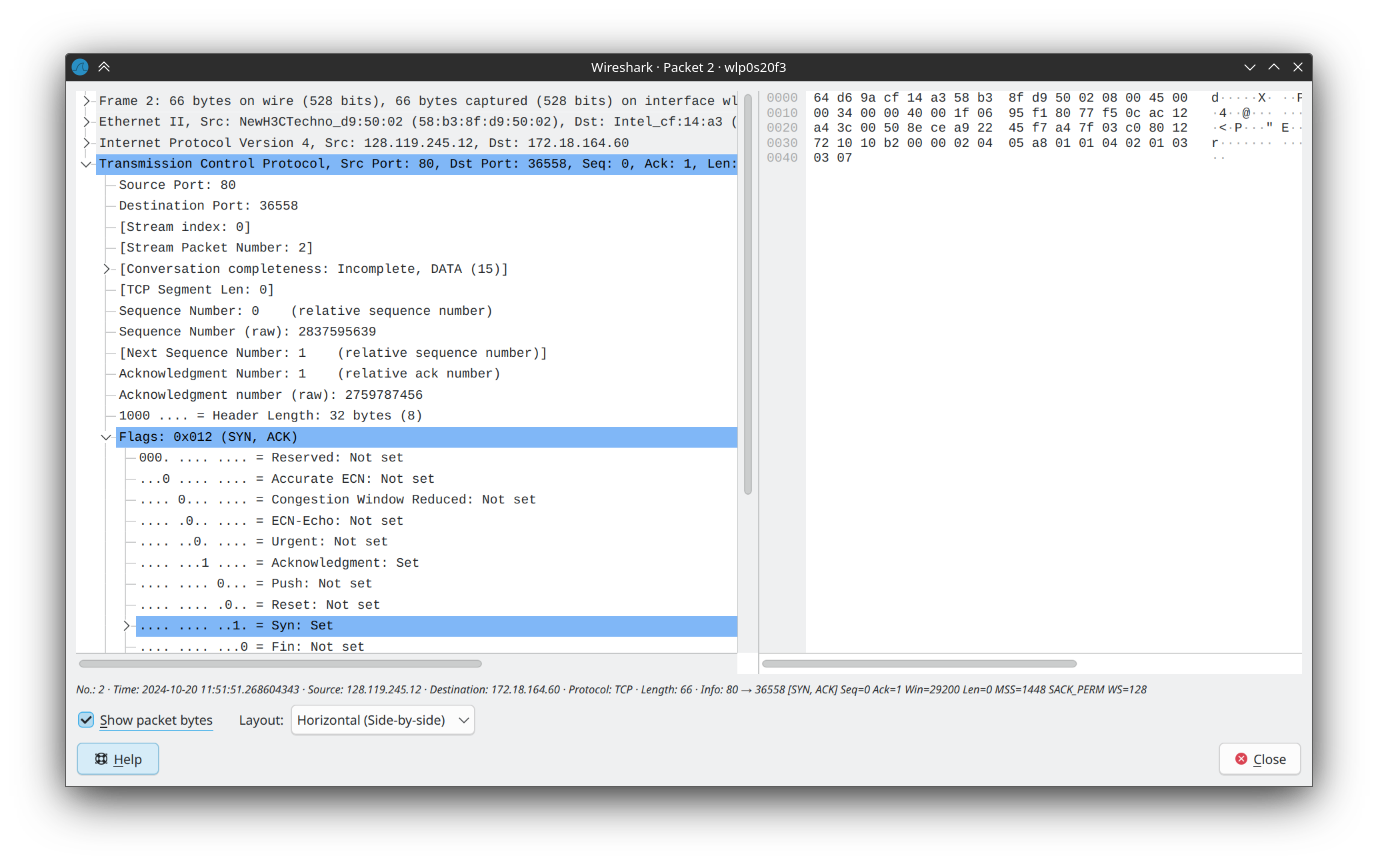
\includegraphics[width=0.8\textwidth]{./lab3-3.png}
    \caption{SYNACK packet}
    \label{fig:SYNACK}
\end{figure}

The \texttt{SYN,ACK} packet is shown in Fig.~\ref{fig:SYNACK}. The \textbf{sequence number is \texttt{2837595639} and the Acknowledgement field is \texttt{2759787456}.} The server determined the value by adding 1 to the sequence number of the SYN packet. The flag is set to \texttt{0x012} which \texttt{SYN} and \texttt{ACK} flags are set.

\subsection*{Question 6.}
\begin{quote}
    What is the sequence number of the TCP segment containing the HTTP POST
    command? Note that in order to find the POST command, you'll need to dig into the packet content field at the bottom of the Wireshark window, looking for a segment with a “POST” within its DATA field.
\end{quote}

\begin{figure}[htbp]
    \centering
    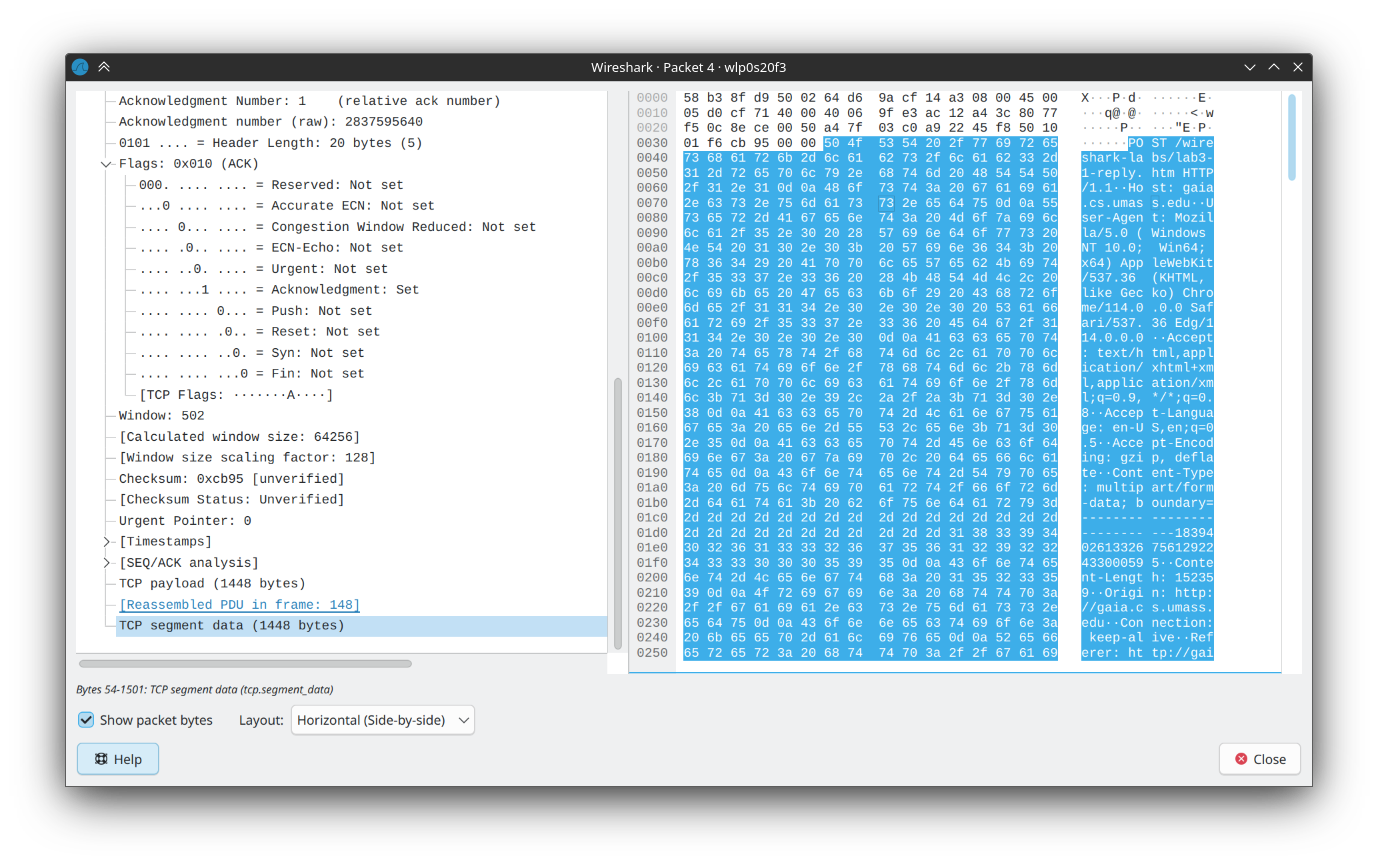
\includegraphics[width=0.8\textwidth]{./lab3-4.png}
    \caption{POST packet}
    \label{fig:POST}
\end{figure}

Inspecting the first TCP packet after the handshake, the details are shown in Fig.~\ref{fig:POST}. The \textbf{sequence number is \texttt{2759787456}}. We can see the \texttt{POST} command at the start of the DATA field.


\subsection*{Question 7.}
\begin{quote}
    Consider the TCP segment containing the HTTP POST as the first segment in the TCP connection. What are the sequence numbers of the first six segments in the TCP connection (including the segment containing the HTTP POST)? At what time was each segment sent? When was the ACK for each segment received? Given the difference between when each TCP segment was sent, and when its acknowledgement was received, what is the RTT value for each of the six segments? What is the \texttt{EstimatedRTT} value (see Section 3.5.3, page 242 in text) after the receipt of each ACK? Assume that the value of the \texttt{EstimatedRTT} is equal to the measured RTT for the first segment, and then is computed using the \texttt{EstimatedRTT} equation on page 242 for all subsequent
    segments.
\end{quote}

\begin{figure}[htbp]
    \centering
    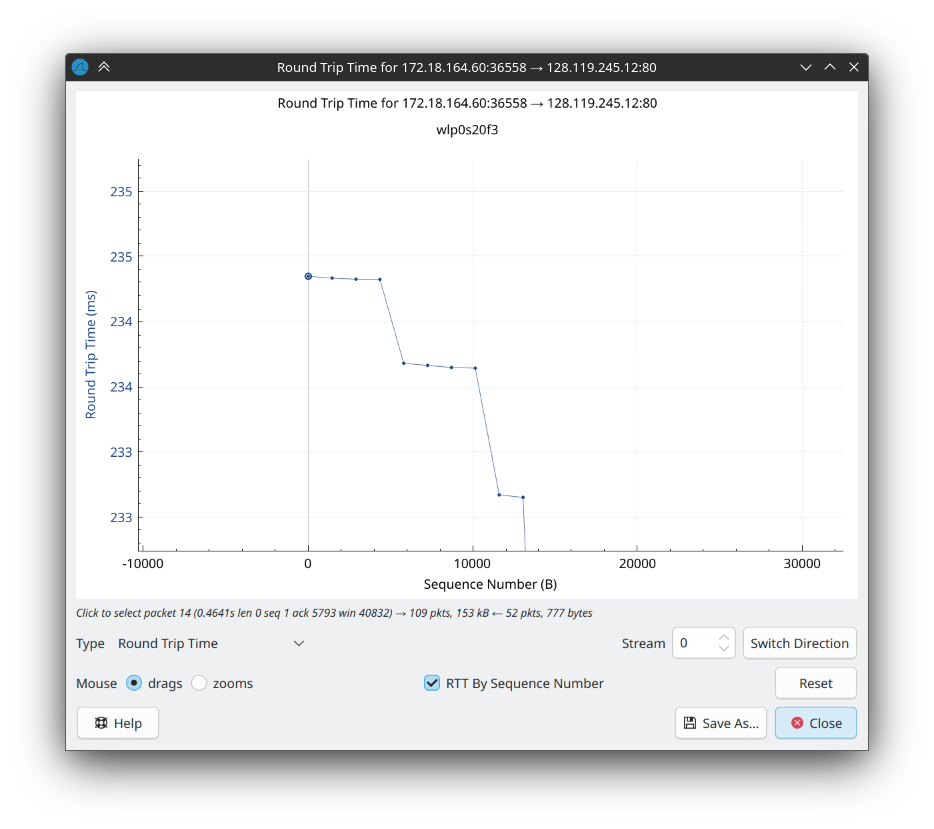
\includegraphics[width=0.8\textwidth]{./lab3-5.png}
    \caption{RTT statistic}
    \label{fig:RTT}
\end{figure}

\begin{figure}[htbp]
    \centering
    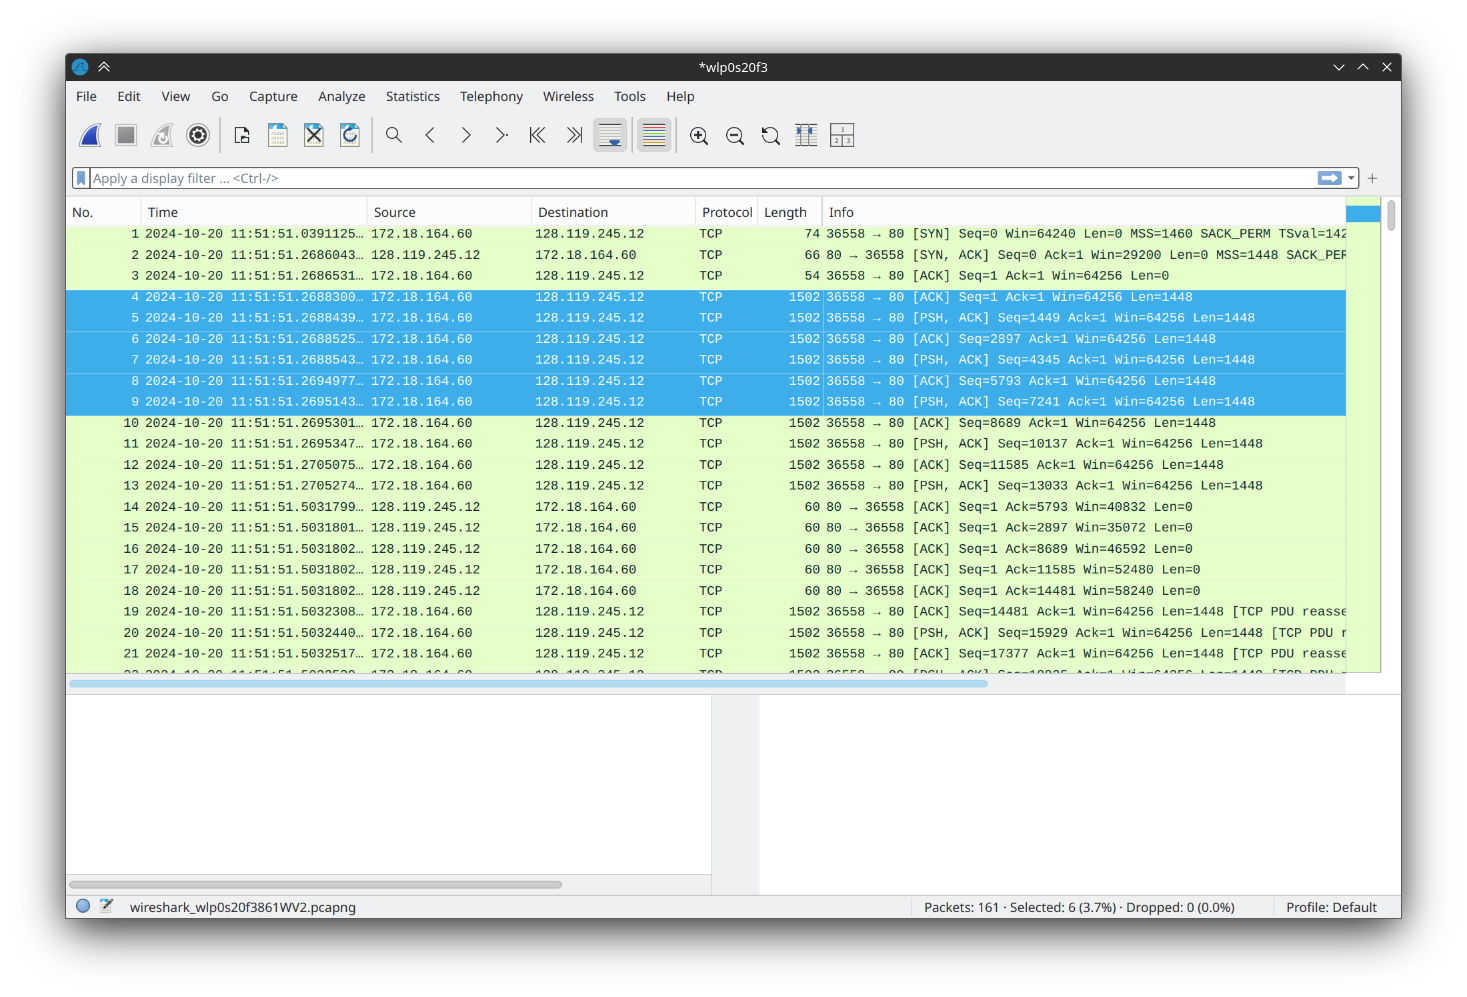
\includegraphics[width=0.8\textwidth]{./lab3-6.png}
    \caption{First 6 packets}
    \label{fig:6packets}
\end{figure}

Using the statistics feature in Wireshark, the RTT statistics are shown in Fig.~\ref{fig:RTT}, and the \texttt{EstimatedRTT} is presented in Fig.~\ref{tab:EstimatedRTT}.

Since the absolute sequence number is not important, we use relative sequence numbers instead.

\paragraph{a.} The sequence numbers of the first six segments are \texttt{1}, \texttt{1449}, \texttt{2897}, \texttt{4345}, \texttt{5793}, and \texttt{7241}. Each one equals the previous sequence number plus the length of the previous segment, which is \texttt{1448}. The details are shown in Fig.~\ref{fig:6packets} with the selected packets.

\paragraph{b\&c.} The time of each segment and its corresponding ACK is shown in Tab.~\ref{tab:time} and Fig.~\ref{fig:RTT}.


\begin{table}[htbp]
    \centering
    \caption{Time of each segment and its ack}
    \label{tab:time}
    \begin{tabular}{cccc}
        \toprule
        Segment & Sent Time                     & Ack Time                      & RTT (ms)   \\
        \midrule
        1       & 2024-10-20 11:51:51.268830094 & 2024-10-20 11:51:51.503179933 & 234.349839 \\
        2       & 2024-10-20 11:51:51.268843992 & 2024-10-20 11:51:51.503179933 & 234.335941 \\
        3       & 2024-10-20 11:51:51.268852535 & 2024-10-20 11:51:51.503179933 & 234.327398 \\
        4       & 2024-10-20 11:51:51.268854358 & 2024-10-20 11:51:51.503179933 & 234.325575 \\
        5       & 2024-10-20 11:51:51.269497706 & 2024-10-20 11:51:51.503180205 & 233.682499 \\
        6       & 2024-10-20 11:51:51.269514380 & 2024-10-20 11:51:51.503180205 & 233.665825 \\
        \bottomrule
    \end{tabular}
\end{table}

We can caluclated the \texttt{EstimatedRTT} using the formula
\[
    \texttt{EstimatedRTT} = (1 - \alpha) \times \texttt{EstimatedRTT} + \alpha \times \texttt{SampleRTT}
\]
where $\alpha = 0.125$.

The \texttt{EstimatedRTT} is shown in Tab.~\ref{tab:EstimatedRTT}

\begin{table}[htbp]
    \centering
    \caption{EstimatedRTT}
    \label{tab:EstimatedRTT}
    \begin{tabular}{cc}
        \toprule
        Segment & EstimatedRTT (ms) \\
        \midrule
        1       & 234.349839        \\
        2       & 234.348102        \\
        3       & 234.345514        \\
        4       & 234.343021        \\
        5       & 234.260456        \\
        6       & 234.186127        \\
        \bottomrule
    \end{tabular}
\end{table}

\subsection*{Question 8.}
\begin{quote}
    What is the length of each of the first six TCP segments?
\end{quote}

From Fig.~\ref{fig:6packets}, we can see the length of each segment is \texttt{1448} bytes.

\subsection*{Question 9.}
\begin{quote}
    What is the minimum amount of available buffer space advertised at the received for the entire trace? Does the lack of receiver buffer space ever throttle the sender?
\end{quote}

\begin{figure}[htbp]
    \centering
    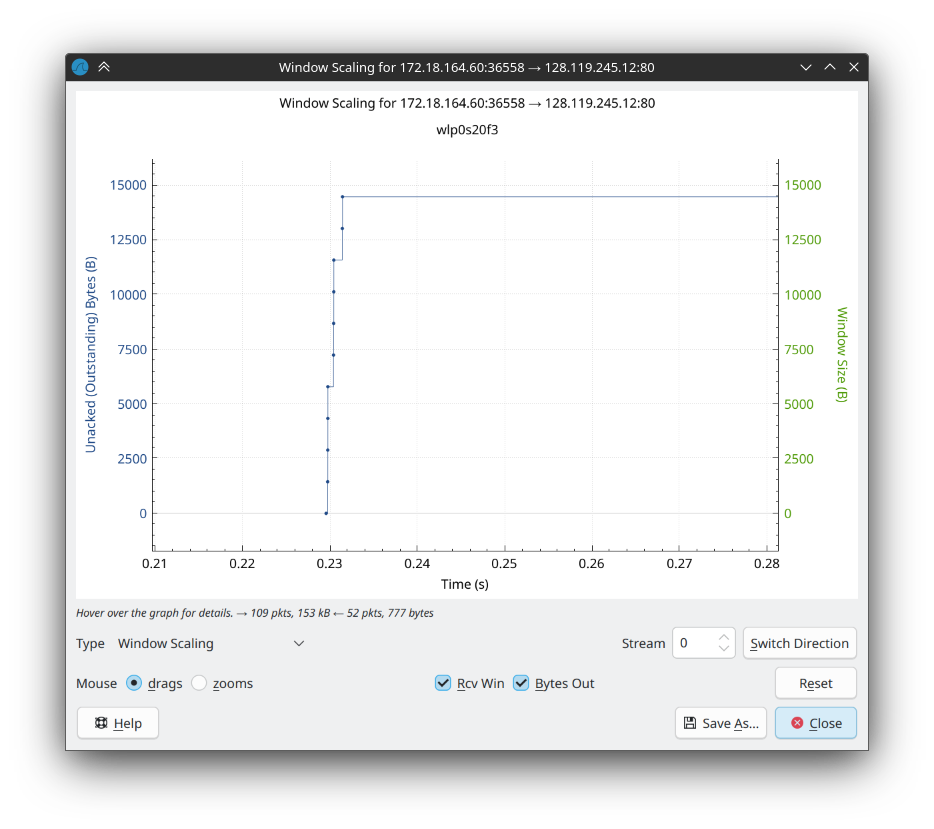
\includegraphics[width=0.8\textwidth]{./lab3-7.png}
    \caption{Window Size}
    \label{fig:Window}
\end{figure}

We can use the statistics feature in Wireshark to obtain the window size. The window size is shown in Fig.~\ref{fig:Window}. As we can see, the window size keeps growing, indicating that the lack of receiver buffer space never throttled the sender. The window size details are also presented in Tab.~\ref{tab:Window}.


\begin{table}[htbp]
    \centering
    \caption{Window Size}
    \label{tab:Window}
    \begin{tabular}{cc}
        \toprule
        Segment & Window Size (Bytes) \\
        \midrule
        1       & 1448                \\
        2       & 2896                \\
        3       & 4344                \\
        4       & 5792                \\
        5       & 7240                \\
        6       & 8688                \\
        \bottomrule
    \end{tabular}
\end{table}

\subsection*{Question 10.}
\begin{quote}
    Are there any retransmitted segments in the trace file? What did you check for (in the trace) in order to answer this question?
\end{quote}

\begin{figure}[htbp]
    \centering
    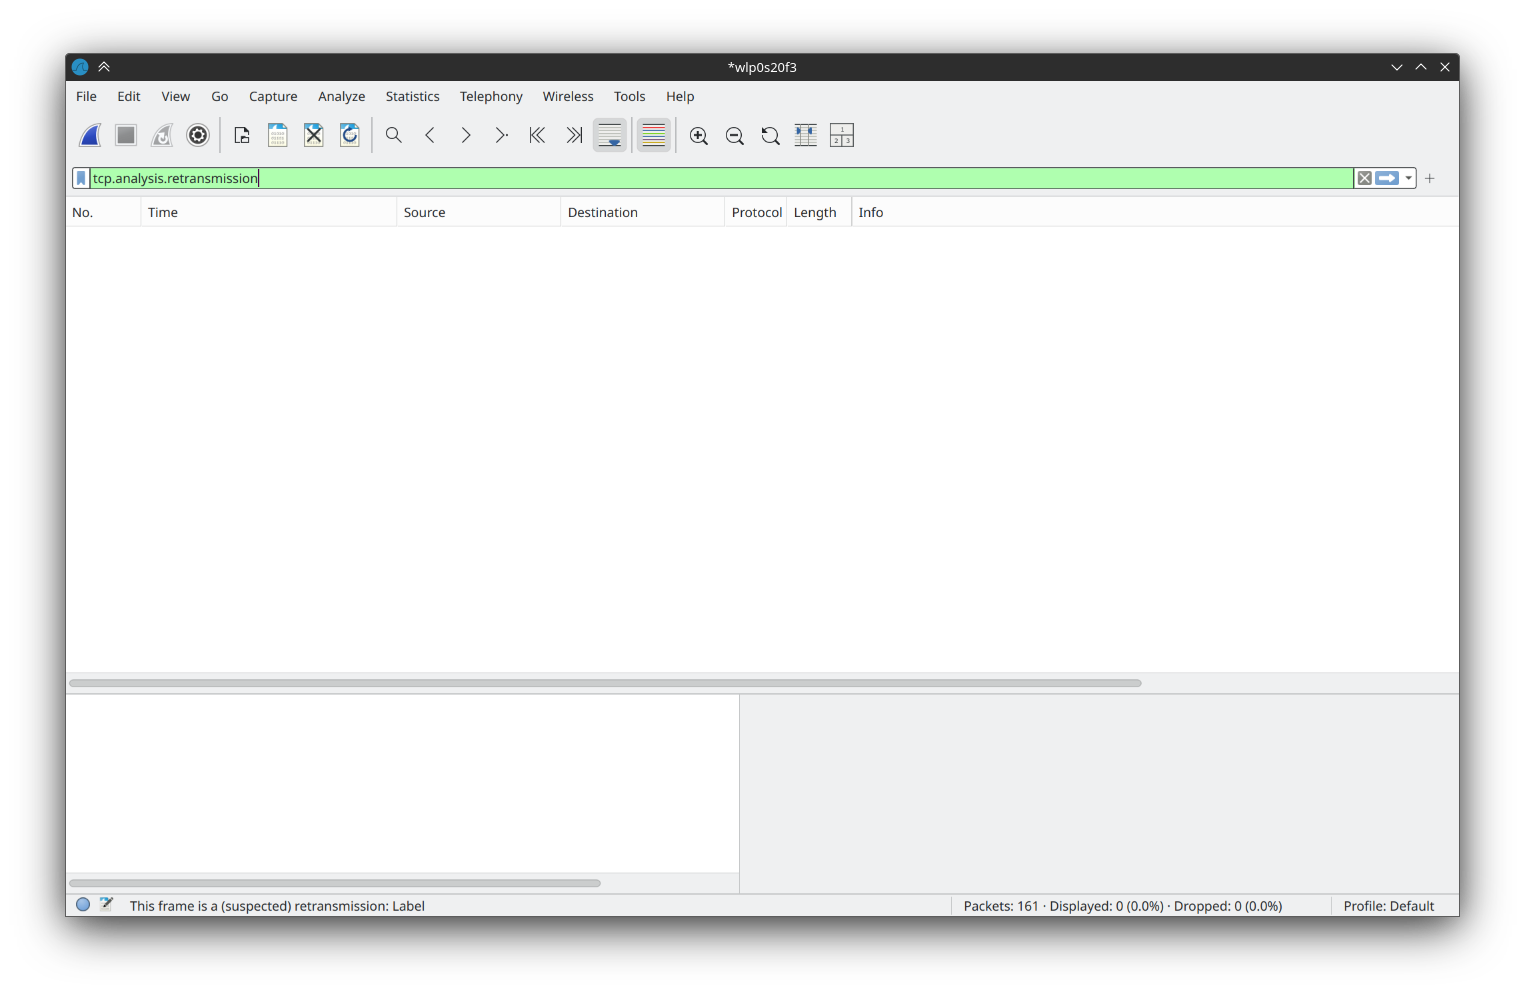
\includegraphics[width=0.8\textwidth]{./lab3-8.png}
    \caption{Retransmission}
    \label{fig:Retransmission}
\end{figure}

We can use the filter \texttt{tcp.analysis.retransmission} to find the retransmitted segments. The result is shown in Fig.~\ref{fig:Retransmission}. As shown, there are no retransmitted segments in the trace.


\subsection*{Question 11.}

\begin{quote}
    How much data does the receiver typically acknowledge in an ACK? Can you identify cases where the receiver is ACKing every other received segment.
\end{quote}

\begin{figure}[htbp]
    \centering
    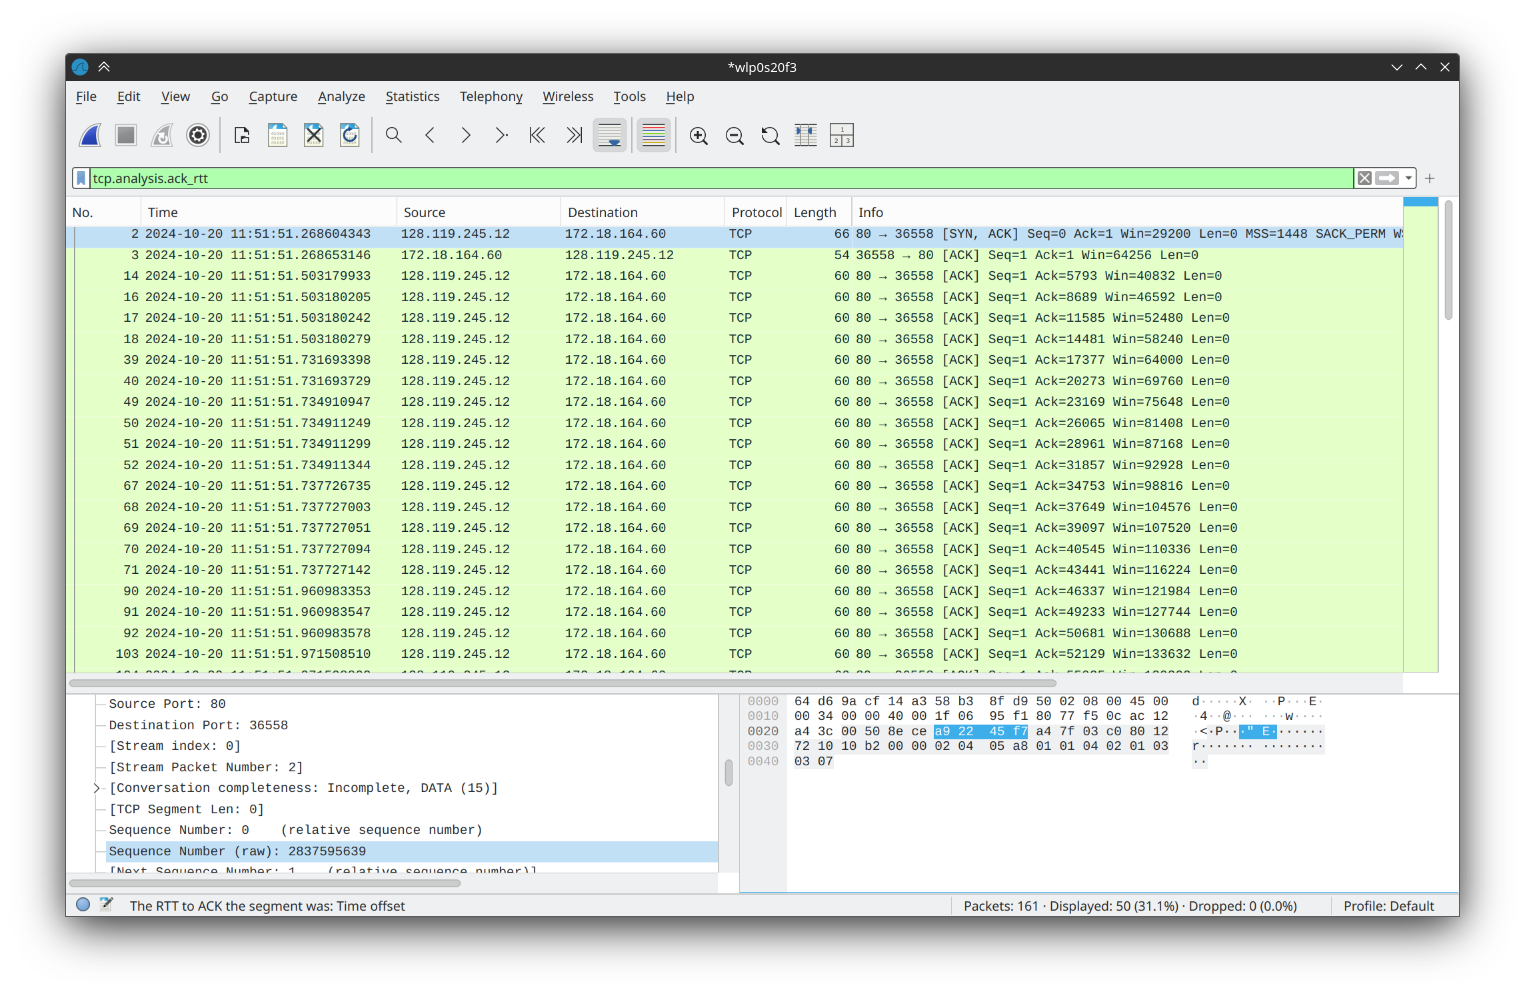
\includegraphics[width=0.8\textwidth]{./lab3-9.png}
    \caption{ACK packets}
    \label{fig:ACK}
\end{figure}


We can use the filter \texttt{tcp.analysis.ack\_rtt} to find the ACK packets. The result is shown in Fig.~\ref{fig:ACK}. We can examine the \texttt{Ack} field to confirm the acknowledgment sequence numbers. The ACK numbers are \texttt{5793}, \texttt{8689}, \texttt{11585}, and \texttt{14481}, among others. This indicates that the \textbf{first ACK acknowledges 5793 bytes, and the subsequent ACKs acknowledge 2896 bytes each}. Fig.~\ref{fig:ACK2} shows the time of each ACK packet, suggesting that there may be delayed ACKs.

\begin{figure}[htbp]
    \centering
    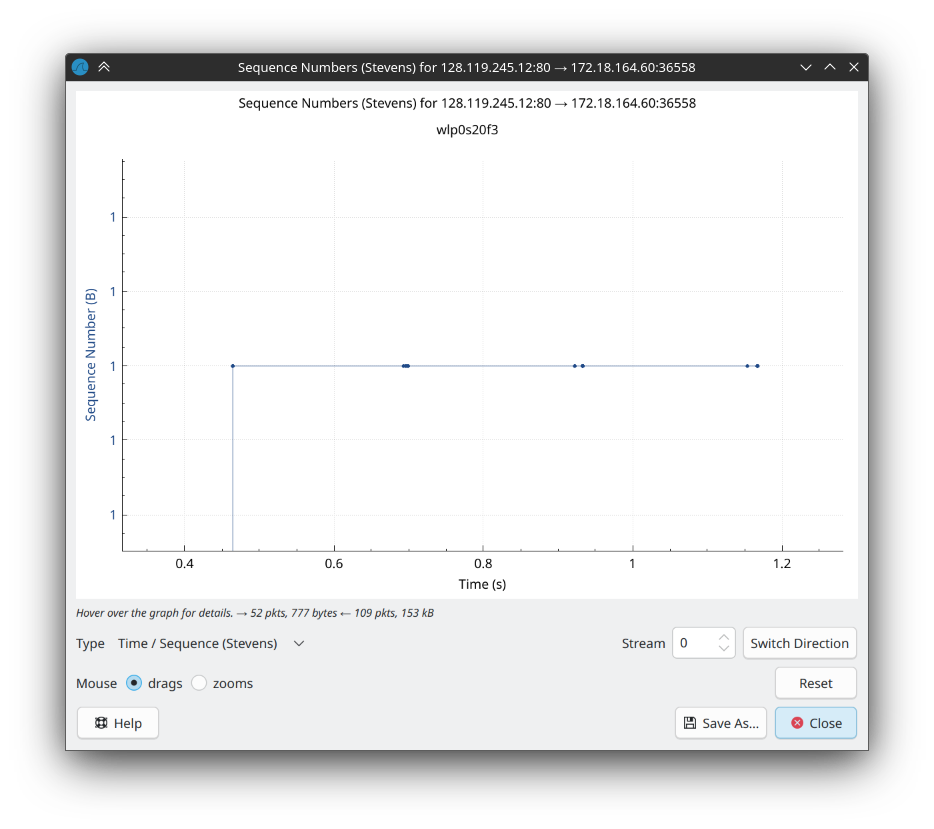
\includegraphics[width=0.8\textwidth]{./lab3-10.png}
    \caption{ACK packets}
    \label{fig:ACK2}
\end{figure}

\subsection*{Question 12.}
\begin{quote}
    What is the throughput (bytes transferred per unit time) for the TCP connection? Explain how you calculated this value.
\end{quote}

\begin{figure}[htbp]
    \centering
    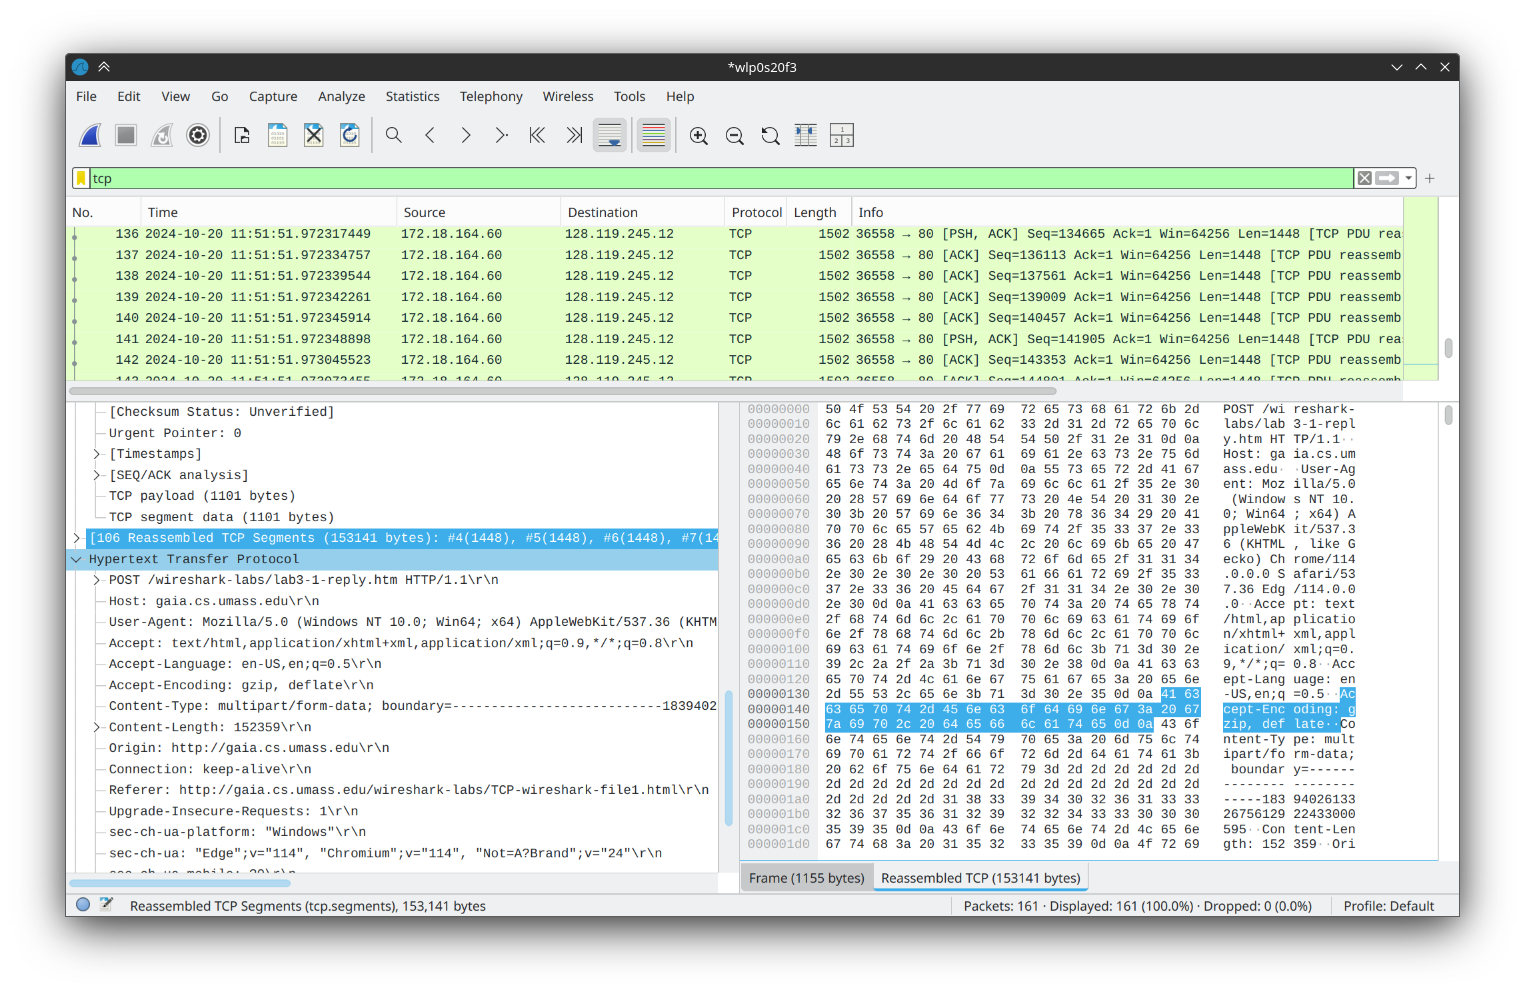
\includegraphics[width=0.8\textwidth]{./lab3-11.png}
    \caption{HTTP request}
    \label{fig:HTTP}
\end{figure}

First, we need to calculate how much data is transferred. By locating the HTTP request, we can see that it indicates the total transferred bytes as 153,141 bytes, as shown in Fig.~\ref{fig:HTTP}.

Next, we calculate the transfer time using the timestamps of the first and last packets. The transfer occurred between 2024-10-20 11:51:51.039112562 and 2024-10-20 11:51:51.973625259, as shown in Fig.~\ref{fig:Uploading} and Fig.~\ref{fig:HTTP}. The transfer time can be calculated as:
\[
    \text{Transfer Time} = 973.625259 - 39.112562 = 934.512697 \text{ms}
\]
Therefore, the throughput is:
\[
    \text{Throughput} =\frac{Bytes Transferred}{Transfer Time} = \frac{153141}{0.934512697} = 163.9 \text{KB/s}
\]

\section{TCP congestion control in action}

\subsection*{Question 13.}

\begin{quote}
    Use the Time-Sequence-Graph(Stevens) plotting tool to view the sequence number versus time plot of segments being sent from the client to the gaia.cs.umass.edu server. Can you identify where TCP’s slowstart phase begins and ends, and where congestion avoidance takes over? Comment on ways in which the measured data differs from the idealized behavior of TCP that we’ve studied in the text.
\end{quote}

\begin{figure}[htbp]
    \centering
    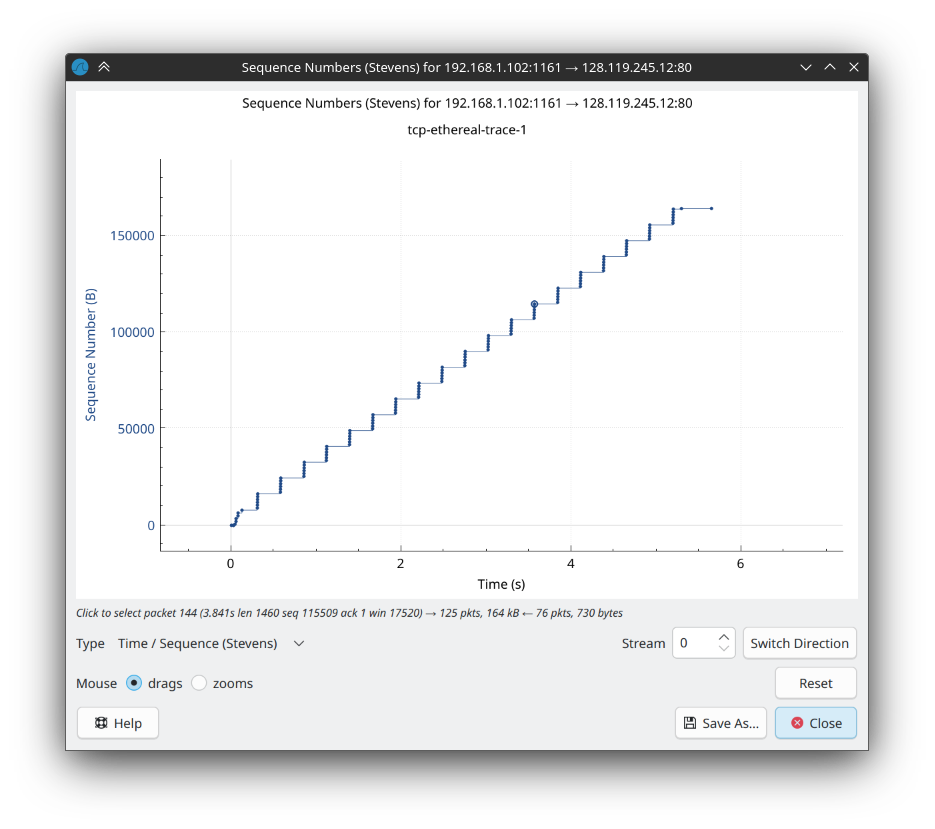
\includegraphics[width=0.8\textwidth]{./lab3-13.png}
    \caption{Time-Sequence-Graph}
    \label{fig:TSG-given}
\end{figure}

From the given trace file, we used the Time-Sequence-Graph to plot the sequence number versus time, as shown in Fig.~\ref{fig:TSG-given}.

The slow start phase begins at the start of the connection and ends around packet 13 at approximately 0.125 seconds. After this point, **congestion avoidance** takes over, but the increase in the congestion window (\texttt{cwnd}) is minimal, and it remains relatively constant for the remainder of the connection.

Compared to the expected behavior, the increase in the congestion window during the congestion avoidance phase is not as pronounced. The \texttt{cwnd} seems to stabilize at a value that is likely best suited for the current network conditions.

\subsection*{Question 14.}

\begin{quote}
    Answer each of two questions above for the trace that you have gathered when you transferred a file from your computer to gaia.cs.umass.ed
\end{quote}


\begin{figure}[htbp]
    \centering
    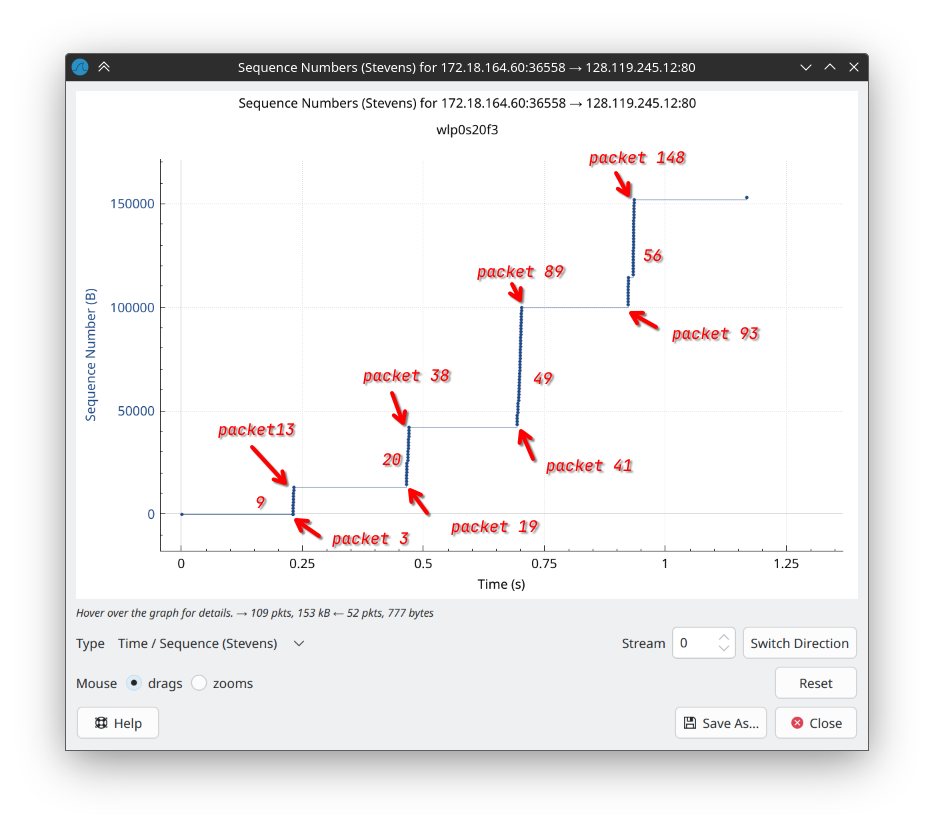
\includegraphics[width=0.8\textwidth]{./lab3-12.png}
    \caption{Time-Sequence-Graph}
    \label{fig:TSG}
\end{figure}

Using the Time-Sequence-Graph, we can observe the sequence number versus time plot of segments being sent from the client to the server. The result is shown in Fig.~\ref{fig:TSG}. The **slow start** phase begins at the start of the connection, with the \texttt{cwnd} increasing almost exponentially from 9 to 49 (though not perfectly exponential). **Congestion avoidance** takes over at packet 93, where the \texttt{cwnd} increases linearly from 49 to 56.

Compared to the expected behavior, the slow start phase is not exactly exponential, and the congestion avoidance phase is not precisely linear either. The \texttt{cwnd} increases in a manner that is less smooth than the idealized behavior.


\end{document}
